\documentclass[11pt]{article} % For LaTeX2e
\usepackage{manuscript, palatino}
\usepackage{graphicx}
\usepackage{amsfonts, amsmath}
\usepackage{algorithm, algpseudocode}%

\usepackage{natbib}

\title{Anxiety: a decision-theoretic perspective}

\author{
Samuel Zorowitz \\
Princeton Neuroscience Institute\\
Princeton University\\
Princeton, NJ 08540 \\
\texttt{zorowitz@princeton.edu} \\
\And
Ida Momennejad \\
Columbia University\\
New York, NY 10027 \\
\texttt{ida.m@columbia.edu} \\
\And
Nathaniel Daw \\
Princeton Neuroscience Institute\\
Princeton University\\
Princeton, NJ 08540 \\
\texttt{ndaw@princeton.edu} \\
}

\newcommand{\fix}{\marginpar{FIX}}
\newcommand{\new}{\marginpar{NEW}}

\begin{document}

\maketitle

\begin{abstract}
To be filled in
\end{abstract}

\keywords{
reinforcement learning; avoidance; anxiety
}

\startmain

\section{Introduction}

Central to many psychiatric disorders is distortion to representations of the
external world and, correspondingly, pronounced changes to learning and decision
making. As a normative framework, decision theory allows us to describe and pose
quantita­tive questions about optimal choice behavior \citep{DayanDaw2008} and is,
therefore, a critical tool for modeling, understanding, and predicting the psychological
and neurobiological mechanisms underlying psychiatric behavior \citep{maia2011, HuysDawDayan2015}.
Recent investigations employing this framework have provided novel and important
insights into psychiatric symptoms and disorders, including anhedonia in major depression \citep{Rutledge2017},
mood instability in bipolar disorder \citep{EldarNiv2015, EldarDolanNiv2016},
habitual behavior in obsessive compulsive and addictive disorders \citep{gillan2016}, and
hallucinations in schizophrenia \citep{powers2017, corlett2018}.

The family of anxiety disorders (which includes generalized anxiety disorder, social
anxiety disorder, panic disorder, and specific phobia) are characterized by excessive
fear and worry about future negative outcomes, and represent the most common
group of psychiatric disorders \citep{kessler2009}. Though the disorders typically
differ in the types of objects or situations that induce fear or anxiety, all share
a set of core disturbances to cognition and behavior. First, the anxiety disorders
involve pessimistic inference, or a tendency to appraise threatening objects or
situations as more likely and/or more severe than they objectively are. Clinical
anxiety is also associated with second-order conditioning, or learning to fear
neutral cues indirectly associated with threat cues. Finally, anxiety is associated
with sustained avoidance, or the tendency for individuals to flee or avoid threatening
situations. As an example, an individual is mugged in an alleyway. In a pathological
response, this individual may exhibit persistent worry that it will happen again
(pessimistic inference), increased anxiety towards the street or time of day
at which it occurred (second-order conditioning), and increased effort to stay
away from any cue which reminds them of the event (avoidance).

Several studies have attempted to provide some insight into why some of this
may be in anxiety disorders \cite{Maia2010, norbury2018}, though no account has
tied these symptoms together. For example, \citep{Maia2010} provided a simple
account of how simple actor-critic reinforcement learning models could account
for sustained avoidance in rodent shuttle-box experiments \citep{servatius2008}.
As has been discussed elsewhere \citep{Moutoussis2017}, such an account fails to account for why avoidance
is maintained even with non-threatening outcomes and do not account for why exposure
therapy only works for some individuals. Other accounts have attempted to explain
pessimistic inference (cite learning rate), but do not mention where from.

In the remainder of this article, we present a simple decision theoretic account
of how the core symptoms of anxiety may arise and be maintained. Specifically, we
demonstrate that the loss of optimistic inference in the form of reduced expectations
of future reward can yield negatively biased estimates of value in sequential
decision environments. In such an event, pessimistic inference, second-order
conditioning, and chronic avoidance naturally follow.

\section{Methods}

\subsection{Markov Decision Processes}

Before moving forward, we first briefly review the formalism of Markov decision
processes, which provide the framework for our results. For complete treatments,
see \cite{SuttonBarto1998, SuttonBarto2018} and \cite{bertsekas2005}.

A MDP is defined by a set of states, $S$, a set of actions, $A$, a reward
function defined over state/action pairs, $R(s,a)$, and a state transition distribution,
$P(s'|s,a)$, where $a$ denotes a chosen action. In a MDP, states and rewards occur
sequentially according to the one-step transition structure where transitions follow
actions. The goal for an agent in a MDP is to learn to choose a policy, $\pi$, or
mapping of state to action, that maximizes long-run expected reward. Here we define
the value of a state under a policy, $V^\pi(s)$, as the expected cumulative discounted reward:

$$ V^\pi(s) = \mathbb{E} \left[ \sum^{\infty}_{k=0} \gamma^k R_{t+k} | S_t = s \right] $$

where $\gamma$ is the temporal discounting parameter, controlling the weighting
of distant future rewards. The value function can be defined recursively as the
sum of the immediate reward following an action chosen in a state, $R(s, a)$, and
the value of its successor state $s’$, averaged over potential future actions, $a$,
and transitions according to the current policy $\pi$:

$$ V^\pi(s) = \sum_a \pi(a|s) \sum_{s',r}p(s',r|s,a) \left[ r + \gamma v(s') \right] $$

Under the optimal policy, the value function is given by:

$$ V^*(s) = \max_a \mathbb{E} \left[ \sum^{\infty}_{k=0} \gamma^k R_{t+k} | S_t = s \right] $$

$$ = \max_a \sum_{s',r}p(s',r|s,a) \left[ r + \gamma v_*(s') \right] $$

Using the formalisms above, the value of one particular action in a state under
the optimal policy is defined as:

$$ Q^\pi(s,a) = \mathbb{E} \left[ \sum^{\infty}_{k=0} \gamma^k R_{t+k} | S_t = s \right] $$

$$ = \sum_{s',r}p(s',r|s,a) \left[ r + \gamma v_*(s') \right] $$

Insofar that the value of a state under the optimal policy is defined as the best
action under that state, we can re-express the above equivalently as:

$$ q_*(s,a) = \sum_{s',r}p(s',r|s,a) \left[ r + \gamma \max_{a'} q_*(s',a') \right] $$

Thus in a conventional MDP, the value of states in the environment under the optimal
policy assumes the agent is able to act according to the optimal policy in the future.

\subsection{Pessimistic Learning}

In the previous section, we observed that the value of a state and its associated
state-action pairs are a function of the environment transition distribution and
the best future action. In standard MDP problems, it is typically assumed that the
transition distribution is known and accurate, and that the agent is consistently
able to operate under the optimal policy in the future. In this section, we introduce
a formalism deviating from these standard assumptions.

Central to many theories of clinical anxiety is a perceived loss of control (see
discussion for elaboration). In the MDP framework described above, this may come
in one of several forms. First, an agent may perceive the transition structure
of the environment to be less reliable than it actually is. Put another way, an
agent may have a biased expectation that, despite choosing an action $a$ with the
intent of transition to state $s'$, the agent may instead transition to an alternate,
undesired state $s^$. In the case of clinical anxiety, the expectation may be more
dire, that the environment is "adversarial" is likely to transition an agent, not
randomly, but to the worse states.

Second, an agent may doubt its own agentive control. An agent may expect to be
able to choose the best possible action for itself in the present, but may not be
confident it will still be able to decide optimally for itself in the future. In
either event, following the value computations defined above, we should expect
the value estimates for such an agent to diminish. If an agent believes itself
or the environment to be unreliable, then the agent cannot be optimistic about
its future and should instead adopt a different policy.

These sorts of problems have been explored in the safe reinforcement learning
and robust control literature \citep{Garcia2015}. There, we are concerned
with programming agents that identify the optimal policy under pessimistic
assumptions. A number of approaches have been proposed in that literature. Here,
we focus on one particular simple implemented proposed by \cite{Gaskett2003}, namely
*w-pessimism*:

$$ V(s') = w \max_{a'} q(s',a') + (1 - w) \min_{a'} q(s',a') $$

such that the state value under the optimal policy is defined as:

$$ V(s) = \max_a \sum_{s',r}p(s',r|s,a) \left[ r + \gamma \left( w \max_{a'} q(s',a') + (1 - w) \min_{a'} q(s',a') \right) \right] $$

In this formalism, $w$ controls the degree of pessimism. When $\w = 1$, an agent
is maximally optimistic and fully expects to act according to the best possible actions
in the future. When $w = 0$, the agent is maximally pessimistic and fully expects
to act according to the worst possible actions in the future. When $w = 0.5$,
the weighs the best and worst possible future actions equally.

We note that we are not committed to this particular implementation of a pessimistic
agent. As mentioned above, an alternative parameterization would have been to
program an agent with a belief in an adversarial environment, preferentially
transitioning it to worse states. Insofar that these two terms are multiplicative
in value calculations, either implementation should yield similar results. Similarly,
the w-pessimism function could easily be replaced with other functions (e.g. softmax
with negative inverse temperature). This formalism is simply convenient and is
useful for demonstrating the points we demonstrate below. It is not a substantive
claim about anxiety.

\subsection{Simulations}

In the following sections, we present the results of simulations of pessimistic
learning in a variety of MDP environments. In all simulations, the state-action
values under the optimal policy, $Q_*(s,a)$, were solved for directly through
Q-value iteration \citep{SuttonBarto1998,SuttonBarto1998,bertsekas2005}. The
details of this algorithm are presented in the appendix. Model parameters are
reported for each environment in their corresponding sections. All simulations
were carried out with the python programming language and are publicly available
on Github (https://github.com/szorowi1/SecretFunTimes).

\section{Results}

\subsection{Pessimistic Inference}

\begin{figure}
  \centerline{%
    \resizebox{1.0\textwidth}{!}{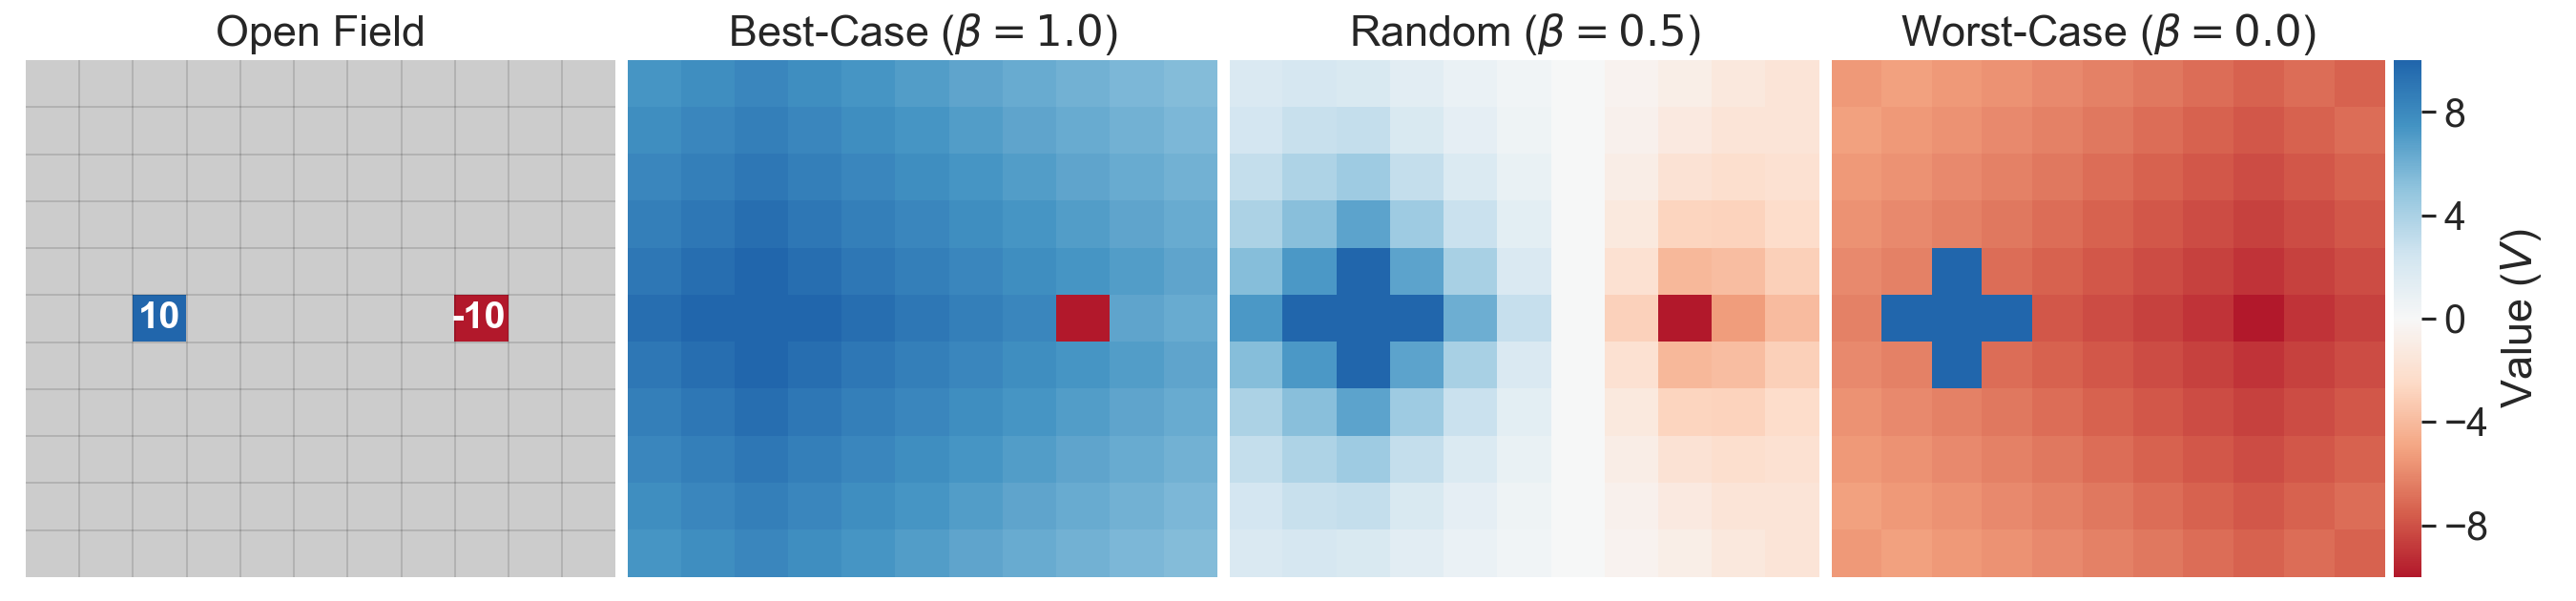
\includegraphics[trim={0 0 0 0},clip]{../figures/01_field.png}}%
  }
  \par Figure 1: The open field environment is a large deterministic gridworld sans one rewarding
  (blue) and aversive (red) state (A). Under optimistic learning conditions (B), all states except
  for the harmful one become positive. Under pessimistic conditions (C), negative value spreads
  from the source to its antecedent states. The extent of the spread is worse for increased
  pessimism (D). (Parameters: $\gamma = 0.95$)
\end{figure}

In this first section, we demonstrate how learning under an assumption of a lack
of future control naturally leads to pessimistic inference and second-order conditioning.
A symptom central to all of the anxiety disorders is pessimistic inference,
or a tendency to appraise the likelihood and/or severity of threatening situations
out of proportion to their actual environmental contingencies \citep{dsm5, BeckClark1997,
ClarkBeck2011}. For example, an individual with specific phobia may vastly exaggerate
the probability of encountering their fear (e.g. a venomous spider) in their
everyday lives. Anxious individuals will also tend to associate fear with cues
tangentially related to signals of threat. For example, the same individual may
begin to fear locations where they may encounter spider webs (e.g. basements).

Pessimistic inference in anxiety is well-documented. In studies of self-reported beliefs,
individuals with anxiety rate
hypothetical future negative outcomes as being more likely to occur and worse to
experience than non-anxious counterparts \citep{ButlerMathews1983, ButlerMathews1987,
Foa1996, MacLeod1996, MacLeod1997, Luten1997, Stober1997, Borkovec1999, Maner2006,
Mitte2007, Miranda2007}. In the laboratory, exaggerated threat appraisal in anxiety
has traditionally been measured through fear conditioning. The results of these
studies demonstrate that anxious individuals exhibit greater fear towards threatening
cues, non-threatening cues, and extinguished threatening cues as compared to non-anxious
counterparts \citep{lissek2005, MinekaOehlberg2008, Duits2015}. Importantly, threatening
cues can become associated with secondary neutral cues, allowing negative value to
spread citep{wessa2007}. In sum, anxiety is associated with inflated estimates of
threat, both likelihood and value, and these estimates can spread from the source
to distantly associated cues.

In our first simulation, we demonstrate how this may come about. In the open field
environment (Figure 1a), an agent is free to navigate a large grid world devoid
of value except for two states: one rewarding and one aversive red. In this environment,
the one-step transition structure is deterministic such that the environment
fully respects the agent's choice. As such, the agent is under no threat despite
the presence of a harmful state. Insofar that the agent never acts under a
masochistic policy and intentionally approaches harm, the agent need not ever
encounter the harmful state.

The long-run value estimates learned by an optimistic agent (i.e. an agent expecting
to be able to follow a reward-maximizing policy now and in the future) reflect this
(Figure 1b). For an optimistic agent, all states in the open field environment,
sans the harmful state itself, take on a positive value. This is unsurprising
insofar that, except for the harmful state, the agent will always encounter
a reward in the long-run no matter its starting position in the field.

The same cannot be said for a the pessimistic agent. If an agent doubts its future
ability to act in according with the optimal policy, then it cannot rule out that,
in the future, it may inadvertently encounter the harmful state. This is more so
likely if the agent is already proximal to the harmful state. Under this pessimistic
belief, the possibility of future harm is no longer zero, as it is for the optimistic
agent, and thus negative value can propagate from the states antecedent to harm,
back to their respective antecedents and so on. The extent of this spread will depend
on the strength of the pessimistic belief (Figures 1c, 1d). With increasing pessimism,
harmful outcomes are assigned greater credence and thus exert greater and wider
influence on antecedent states.

In sequential decision environments then, a perceived lack of self-efficacy can
result in the propagation of negative value from potential future harms. Such a
pessimistic agent may correspondingly report an increased likelihood of threat
(i.e. a greater number of threatening states), increased severity of threat (i.e.
states with more negative value), and fear of states antecedent to the fear source.
As such, pessimistic learning can account for two of the hallmark symptoms of
the anxiety disorders.

\subsection{Avoidance}

A second symptom central to all anxiety disorders is avoidance \citep{dsm5,
Krypotos2015, Arnaudova2017}, or actions taken to increase or maintain the temporal,
physical and/or mental distance between an individual and a threatening situation.
Although avoidance is a natural response to danger, excessive avoidance as is
observed in anxiety disorders is can be highly disruptive to everyday functioning
\cite{Salter2004} and may work to sustain anxious appraisals and behavior. For
example, an individual with social anxiety may avoid attending large social events
for fear of public embarrassment only to never learn that such worry is not justified.

Avoidance is often chosen even at the expense of potential reward (approch-avoidance
conflict), and is frequently a major impediment to recovery \citep{Arnaudova2017}.

In the laboratory, avoidance has been measured in a variety of ways. In animal
models of anxiety, anxious rodents are found to exhibit avoidance learning more
quickly and maintain avoidance for longer \citep{servatius2008}. In studies of
human avoidance, anxiety has been found to correlate with the maintenance of
increased distance from threat, such as virtual predators \citep{Bach2014, Bach2017,
Sheynin2014}.

% Arnaudova2017 makes reference to some spider approach studies that might be
% interesting to try and track down. Essential idea is that even though
% participants are totally safe, may not touch the glass. The task is the
% behavioral avoidance task. (e.g. Siegel & Weinberger, 2012, emotion).
% the nice part about this is that participants are objectively safe.

There is a long history of models attempting to explain avoidance learning. The
fundamental challenge is explaining how an action can be reinforced in the
absence of an outcome. Two-factor theory was the explanation for a long while,
but suffered from a number of noteworthy criticisms \citep{Krypotos2015}.
Recent work has revitalized two-factor theory and integrated it with reinforcement
learning \citep{Moutoussis2008, Maia2010}, and in the process addressing several
criticisms of two-factor theory. As has been discussed elsewhere \citep{Moutoussis2017},
such accounts only explain the maintenance of avoidance in short timescales, but
do not explain why resistant to change and why they do not go away in general.

% Need to go into more detail than this, need to actually make this a coherent
% explanation, but this can wait for now.

\begin{figure}
  \centerline{%
    \resizebox{1.0\textwidth}{!}{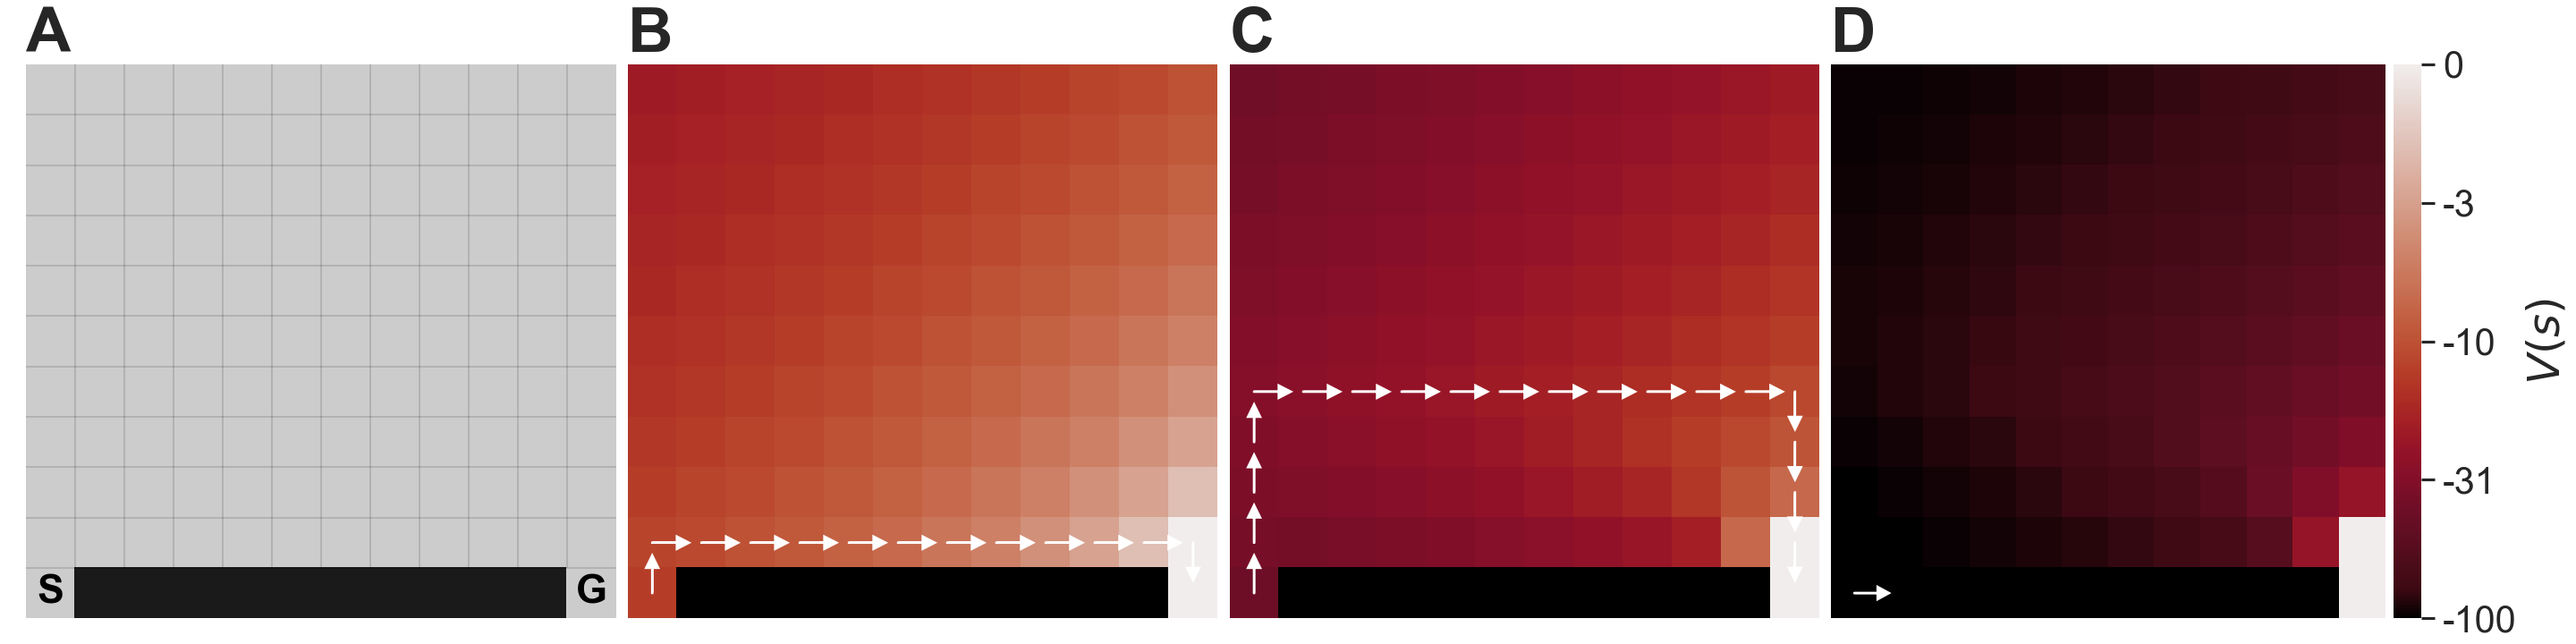
\includegraphics[trim={0 0 0 0},clip]{../figures/02_cliff.png}}%
  }
  \caption{\textbf{Cliff Walking}}
  \par Cliff = -100, Cost = -1, gamma = 0.99
\end{figure}

In our second result, we demonstrate how a breakdown in control can lead to
sustained policies of avoidance. We do so in the cliff-walking environment
\citep{SuttonBarto1998, SuttonBarto2018, Gaskett2003}. Here an agent learns to navigate from
an initial starting position to an end state. The shortest distance is along a
cliff edge. If the agent steps off the cliff, it incurs a large penalty. Under
complete control (objective or perceived), agent in this environment is under no
threat despite the presence of the cliff's edge. As in the first simulation, this
is simply because, in a fully controllable world, an agent need not ever interact
with the aversive state. In fact, an agent can decide to walk straight up to the
aversive state and, insofar it does not choose to take one step further, will
never be in any actual danger.

This is not so when deterministic control cannot be assumed. If an agent believes
it is not in full control of its environment, then it cannot rule out the possibility
that it may inadvertently encounter the negative state at some point in the future,
especially if it veers to close to the state. This is true irrespective of whether
the agent believes it cannot guarantee its own future competency or the benevolence
of the environment. Importantly, this belief need not match the true environmental
statistics; belief is enough.

The long-run state values under different beliefs are plotted in Figure 2. As
expected, under optimistic beliefs (Figure 1b) the entire environment sans negative
state takes on a positive value (close to the positive state itself). As this belief
breaks down, we observe a different pattern in the long-run state values. When
future occupancy of the negative state becomes a non-zero probability, the undesired
action transition exerts influence on action-outcome calculations, back-propagating,
and thereby infecting antecedent states. As the agent's belief becomes increasingly
pessimistic, the more the worst possible action exerts influence and the more
negative, on average, the state-space grows. Most importantly, because these are
the long-run state values, the policy is the optimal policy; in other words, this
is the long-run policy an agent will take.

\subsection{Approach-Avoidance Conflict}

Next, we turn our attention towards a related phenomenon: a bias towards avoidance
in approach-avoidance conflict. In environments with correlated risk and rewards,
a bias towards avoidance can ultimately result in fewer expected rewards and worse
long-run returns. Returning to the example above, an individual with social anxiety
may forgo social situations to avoid the risk of social embarrassment at the expense
of friendships, etc. This is another way in which pathological anxiety can be
disruptive to everyday functioning.

Experimentally, there is a long history of measuring behavior during
approach-avoidance conflict in individuals with anxiety (citation, maybe yin-yang anxiety paper).
One popular paradigm is the balloon analog risk task (BART) \citep{Lejuez2002},
which has been shown to correlate with anxiety \cite{Maner2007, Giorgetta2012}.
In the task, a participant pumps a balloon with air. For each pump, the participant
earns points. If she pumps too much, the balloon pops and she loses all points.
The participant must decide within each episode when to stop pumping. Leave time
is the measure of behavior, with earlier leave times in anxiety suggesting a
greater tendency towards avoidance.

\begin{figure}
  \centerline{%
    \resizebox{1.0\textwidth}{!}{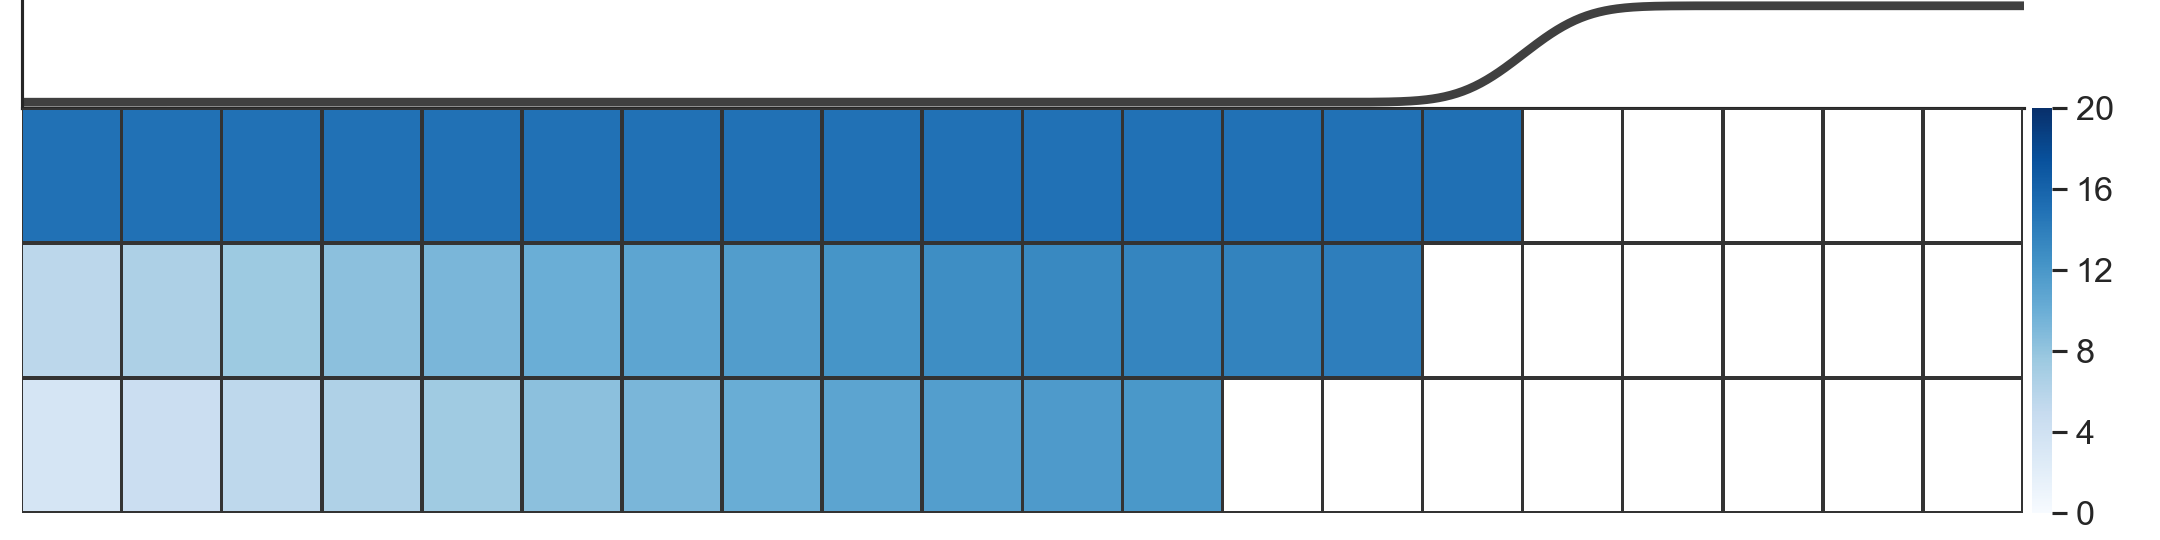
\includegraphics[trim={0 0 0 0},clip]{../figures/03_fid.png}}%
  }
  \caption{\textbf{BART}}
  \par remember to add parameters
\end{figure}

Our sequential model of decision making easily explains these results. A schematic
of the task is presented in Figure 3. Under optimistic beliefs, points should
travel back from the mean. Under pessimistic assumptions, however, different
degrees of the worst outcome backpropagate. At a certain point, the perceived cost
of staying outweighs the guaranteed gains of leaving. Thus, patients with anxiety
leave earlier.

We can explain similar findings with the flight initiation distance \citep{Mobbs2018,
Mobbs2019}. One thing our model cannot explain is the neural difference between
fast and slow escape. Indeed, our model cannot capture all but perhaps is relevant
for certain calculations. One could imagine these beliefs interacting in such a
way to change the distance calculations that are necessary for mediating between
passive and active defense responses.

This can also be used to explain behavioral inhibition \citep{bach2015, khemka2017}.
The idea is slightly different than what is advocated. The claim here is that
in anxious individuals, the Q-values should be closer together, and thus there
should be longer waiting time.

\subsection{Planning}

In this next section, we review the literature on aversive pruning. In large,
multi-step sequential decision environments, the space of all possible sequences
of choices grows exponentially larger with increasing sequence length. As such,
it is infeasible for decision making agents to exhaustively explore all possible
sequences select that which maximizes reward from the entire set. Heuristics for
narrowing the search space then are not only plausible but beneficial for a
decision making agent.

One such heuristic that has been proposed in the literature is aversive pruning
\citep{Huys2012}. Aversive pruning is defined as a Pavlovian response to encountering
a large loss in planning such that sequences involving large losses are discarded
from further evaluation. An example of scenario is presented in Figure 4. The prediction
in such an environment is that an agent would discard the branch of the decision
tree involving an immediate large negative loss even though this branch objectively
contains the reward maximizing (loss minimizing) sequence of choices.

\cite{Huys2012} (and later \cite{Lally2017}) tested this prediction in the
choice envrionment displayed in Figure 4. Participants received extensive training
in this decision tree environment (first without outcomes and then later with
rewards) in order to facilitate planning. In free-planning trials, many participants
exhibited this Pavlovian bias, rejecting choice sequences which involved the large
loss even when the sequence was objectively reward maximizing (loss minimizing).
Importantly \cite{Huys2012} and \cite{Lally2017} found the degree of aversive
pruning was correlated with depressive and anxiety symptoms, respectively.

The aversive pruning principle makes tremendous sense and draws on a robust literature
of heuristics and computational shortcuts for circumventing computationally intractable
cognitive processes. It is important to note, however, that a control interpretation
also makes similar predictions. Figure 4b-d shows the preferred routes of simulated
agents in the same environments under increasingly pessimistic expectations of
future actions. As can be observed, pessimistic agents are similarly likely to avoid
the branch with the large loss, though for different reasons. Under the pessimistic case,
the agent is increasingly less confident that the large gains later in
sequence will be realized; as such, the agent is less confident that the initial
large loss will be offset. Consequently, pessimistic agents would prefer the branch
with smaller losses (even if this is objectively suboptimal). This prediction
is similarly consistent with the finding that avoidance of the initial large loss
is correlated with anxiety \cite{Lally2017}.

An interpretation like this would be consistent with reduced beliefs in one's
own competency in such an environment. This is not strictly surprising. Planning
multi-choice sequences even in relatively simple environments like those used
in these experiments still ostensibly require working memory ability to keep in
mind the possible consequences along each branch. Insofar that working memory
ability is disrupted in anxiety disorders \citep{Moran2016}, a pessimistic belief
may be justified and possibly optimal.

It is also worht noting that the two theories can be easily disentangled with a
simple manipulation of the choice environment. The two theories predict
different choices when the large loss comes later in sequence. For aversive pruning,
late large losses should have little effect on choice behavior. For pessimistic
learning, however, the value of large losses should back-propagate and contaminate
its associated branch. Future experiments can tease these apart as tests of the theory.

\begin{figure}
  \centerline{%
    \resizebox{1.0\textwidth}{!}{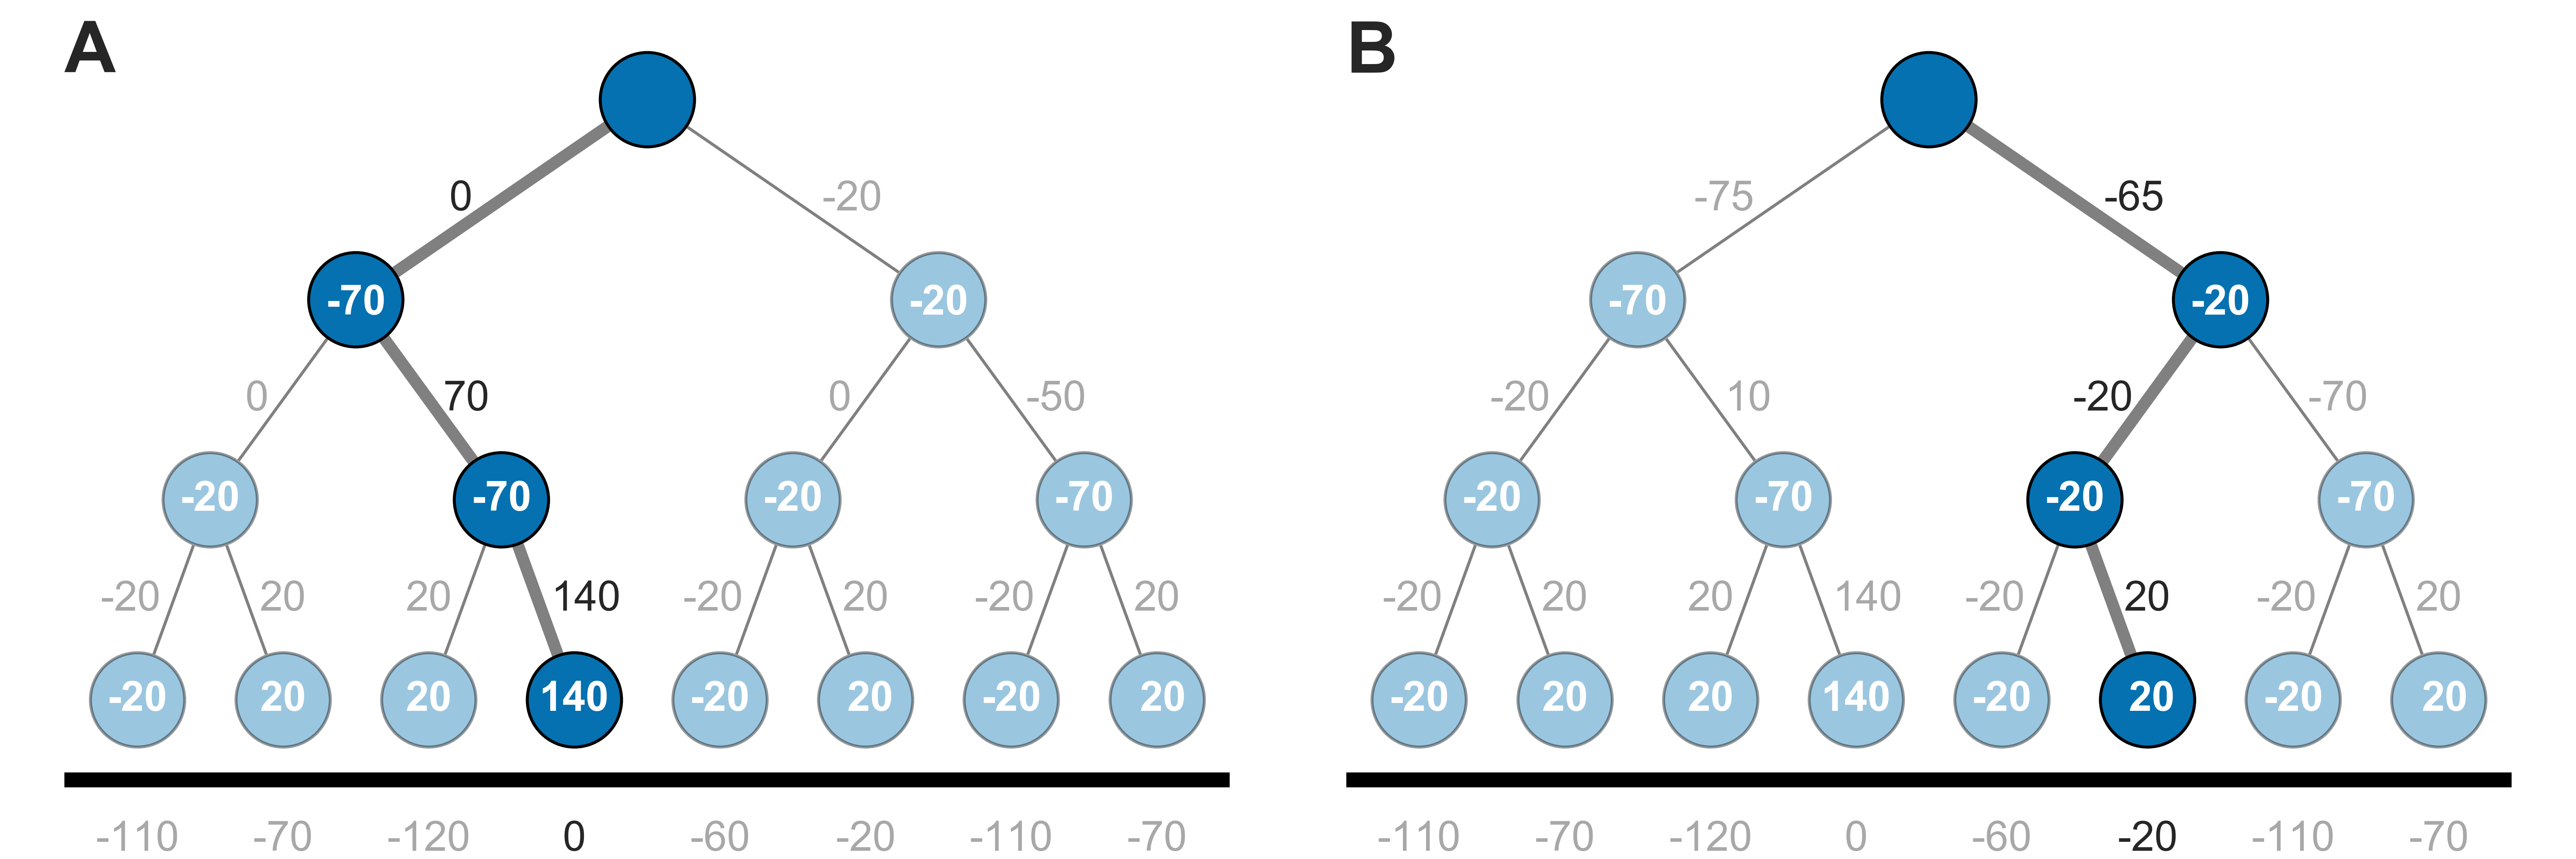
\includegraphics[trim={0 0 0 0},clip]{../figures/04_tree.png}}%
  }
  \caption{\textbf{Decision Tree}}
  \par remember to add parameters
\end{figure}

\subsection{Free Choice Premium}

If an agent is confident that their compentency in decision-making in intact,
then it follows that situations in which an individual is able to make a choice
should be preferable to situations in which an individual is not. At worst,
an agent is no better off than if they had not made a choice; at best, an agent
is better able to steer themselves toward desirable outcomes. Such is the logic
that underlies an increasingly robust literature suggesting choice is inherently
valuable \citep{Leotti2010}.

This free choice premium has been demonstrated multiple times in humans \citep{Suzuki1997,Leotti2011,Leotti2014,Cockburn2014} using a variety of decision
paradigms. For the present purposes, we will describe the experiments presented in
\citep{Leotti2011,Leotti2014}. In these experiments, participants complete a
two-stage decision making task (Figure 5). In the first stage, participants are
make a choice between two cues: one leading to free choice and the other leading
to a fixed choice. In the second stage, participants are able to choose between
a second set of cues (free choice) or are forced to choose a cue (fixed choice).
Unbeknownst to participants, all cues yield reward following the same outcome
distribution; thus, no cue is advantageous in the long-run. The free choice
premium is measured as a preference for the cue leading to free choice. \cite{Leotti2011,Leotti2014}
find participants still prefer the free choice cue, despite this conferring no
objective benefit to participants.

Insofar that this effect is contingent on the belief of one's own competency,
it stands to reason that this free choice premium should be absent in individuals
with anxiety and anxious control beliefs. We demonstrate this effect in Figure 5.
In each trial, the reward outcomes are equal for all options (-1, 1). In individuals
with increasingly pessimistic beliefs, the worst outcome in free choice is increasingly
back-propagated to the free-choice cue, thereby making it less attractive than
the fixed choice cue. Hence, pessimistic learners, on average, do not exhibit
this choice bias.

To our knowledge this prediction has not been empirically tested.

\begin{figure}
  \centerline{%
    \resizebox{1.0\textwidth}{!}{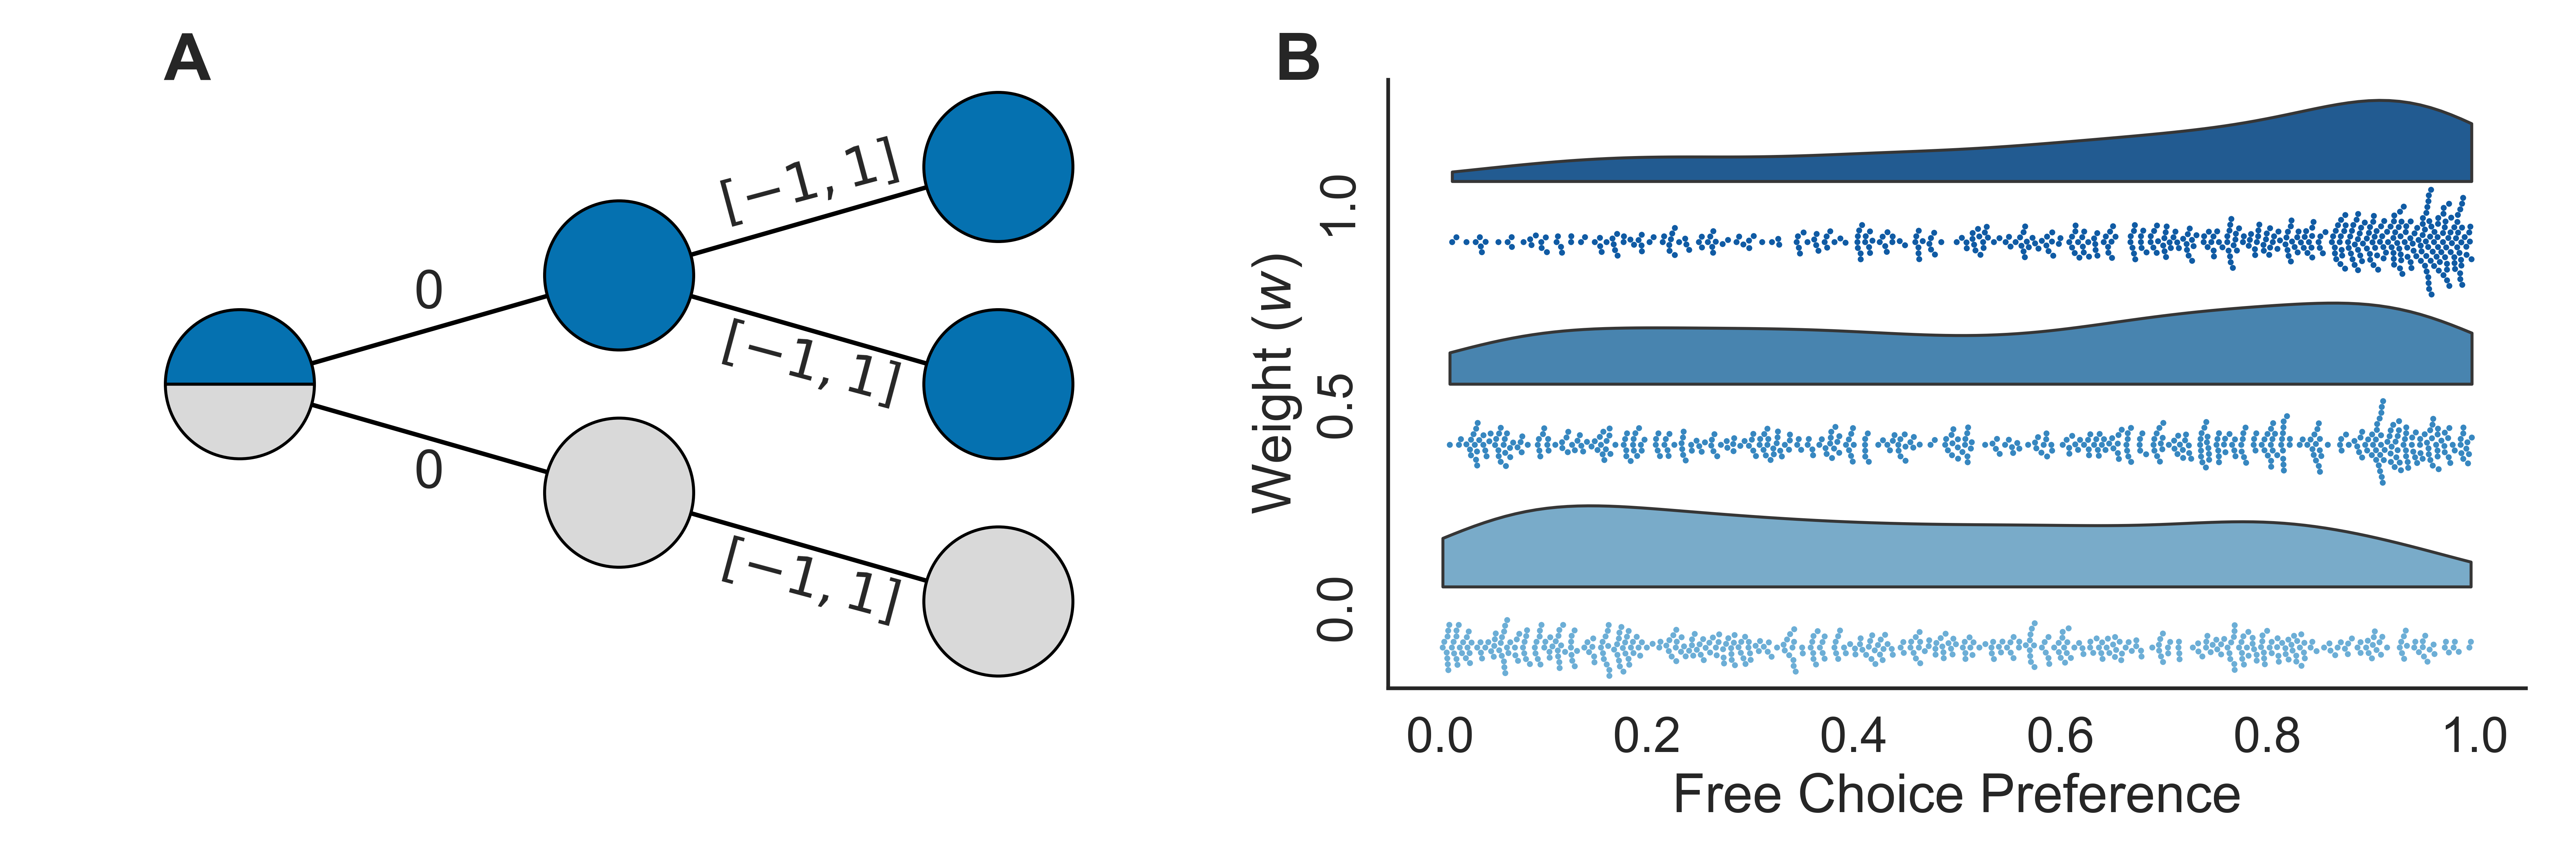
\includegraphics[trim={0 0 0 0},clip]{../figures/05_choice.png}}%
  }
  \caption{\textbf{Free Choice Premium}}
  \par remember to add parameters
\end{figure}

\subsection{Longitudinal Progression}

In this final section, we want to discuss the relationship between anxiety and
depression. Anxiety and depression are highly comorbid, with roughly 45% of individuals
with lifetime depression diagnosis also diagnosed with at least one anxiety disorder
\citep{kessler2015}. This fact has long been recognized in the clinical literature,
and prominent theories of depression have suggested that anxious control is a necessary
precursor to at least some types of depression \citep{alloy1990}. Recent large-scale
epidemiological studies have provided  some empirical support for this claim, finding that
anxiety symptoms precede and predict the onset of depression \citep{mathew2011, jacobson2014,
kessler2015} (though also see \cite{jacobson2017, plana2019}).

An emerging idea in this literature is that pathological avoidance as a result
of anxiety mediates the transition to depression, perhaps by reduce the likelihood
of experiencing positive events and activities \citep{moitra2008, jacobson2014}.
This finding is perfectly in line with the model presented so far. A sketch of
how this is possible is shown in Figure 6. Under unperturbed learning, avoidable
threat does not impede behavior. Under pessimistic learning, threat can block
future reward. This avoidance can manifest as a failure of behavioral initiation,
or a lack of overall mobility (here represented by an agent self-transitioning
at the starting state). Thus, the model can accommodate the deficits in positive
affect observed in depression as a function of behavioral avoidance, as predicted
by these epidemiological studies.

\begin{figure}
  \centerline{%
    \resizebox{1.0\textwidth}{!}{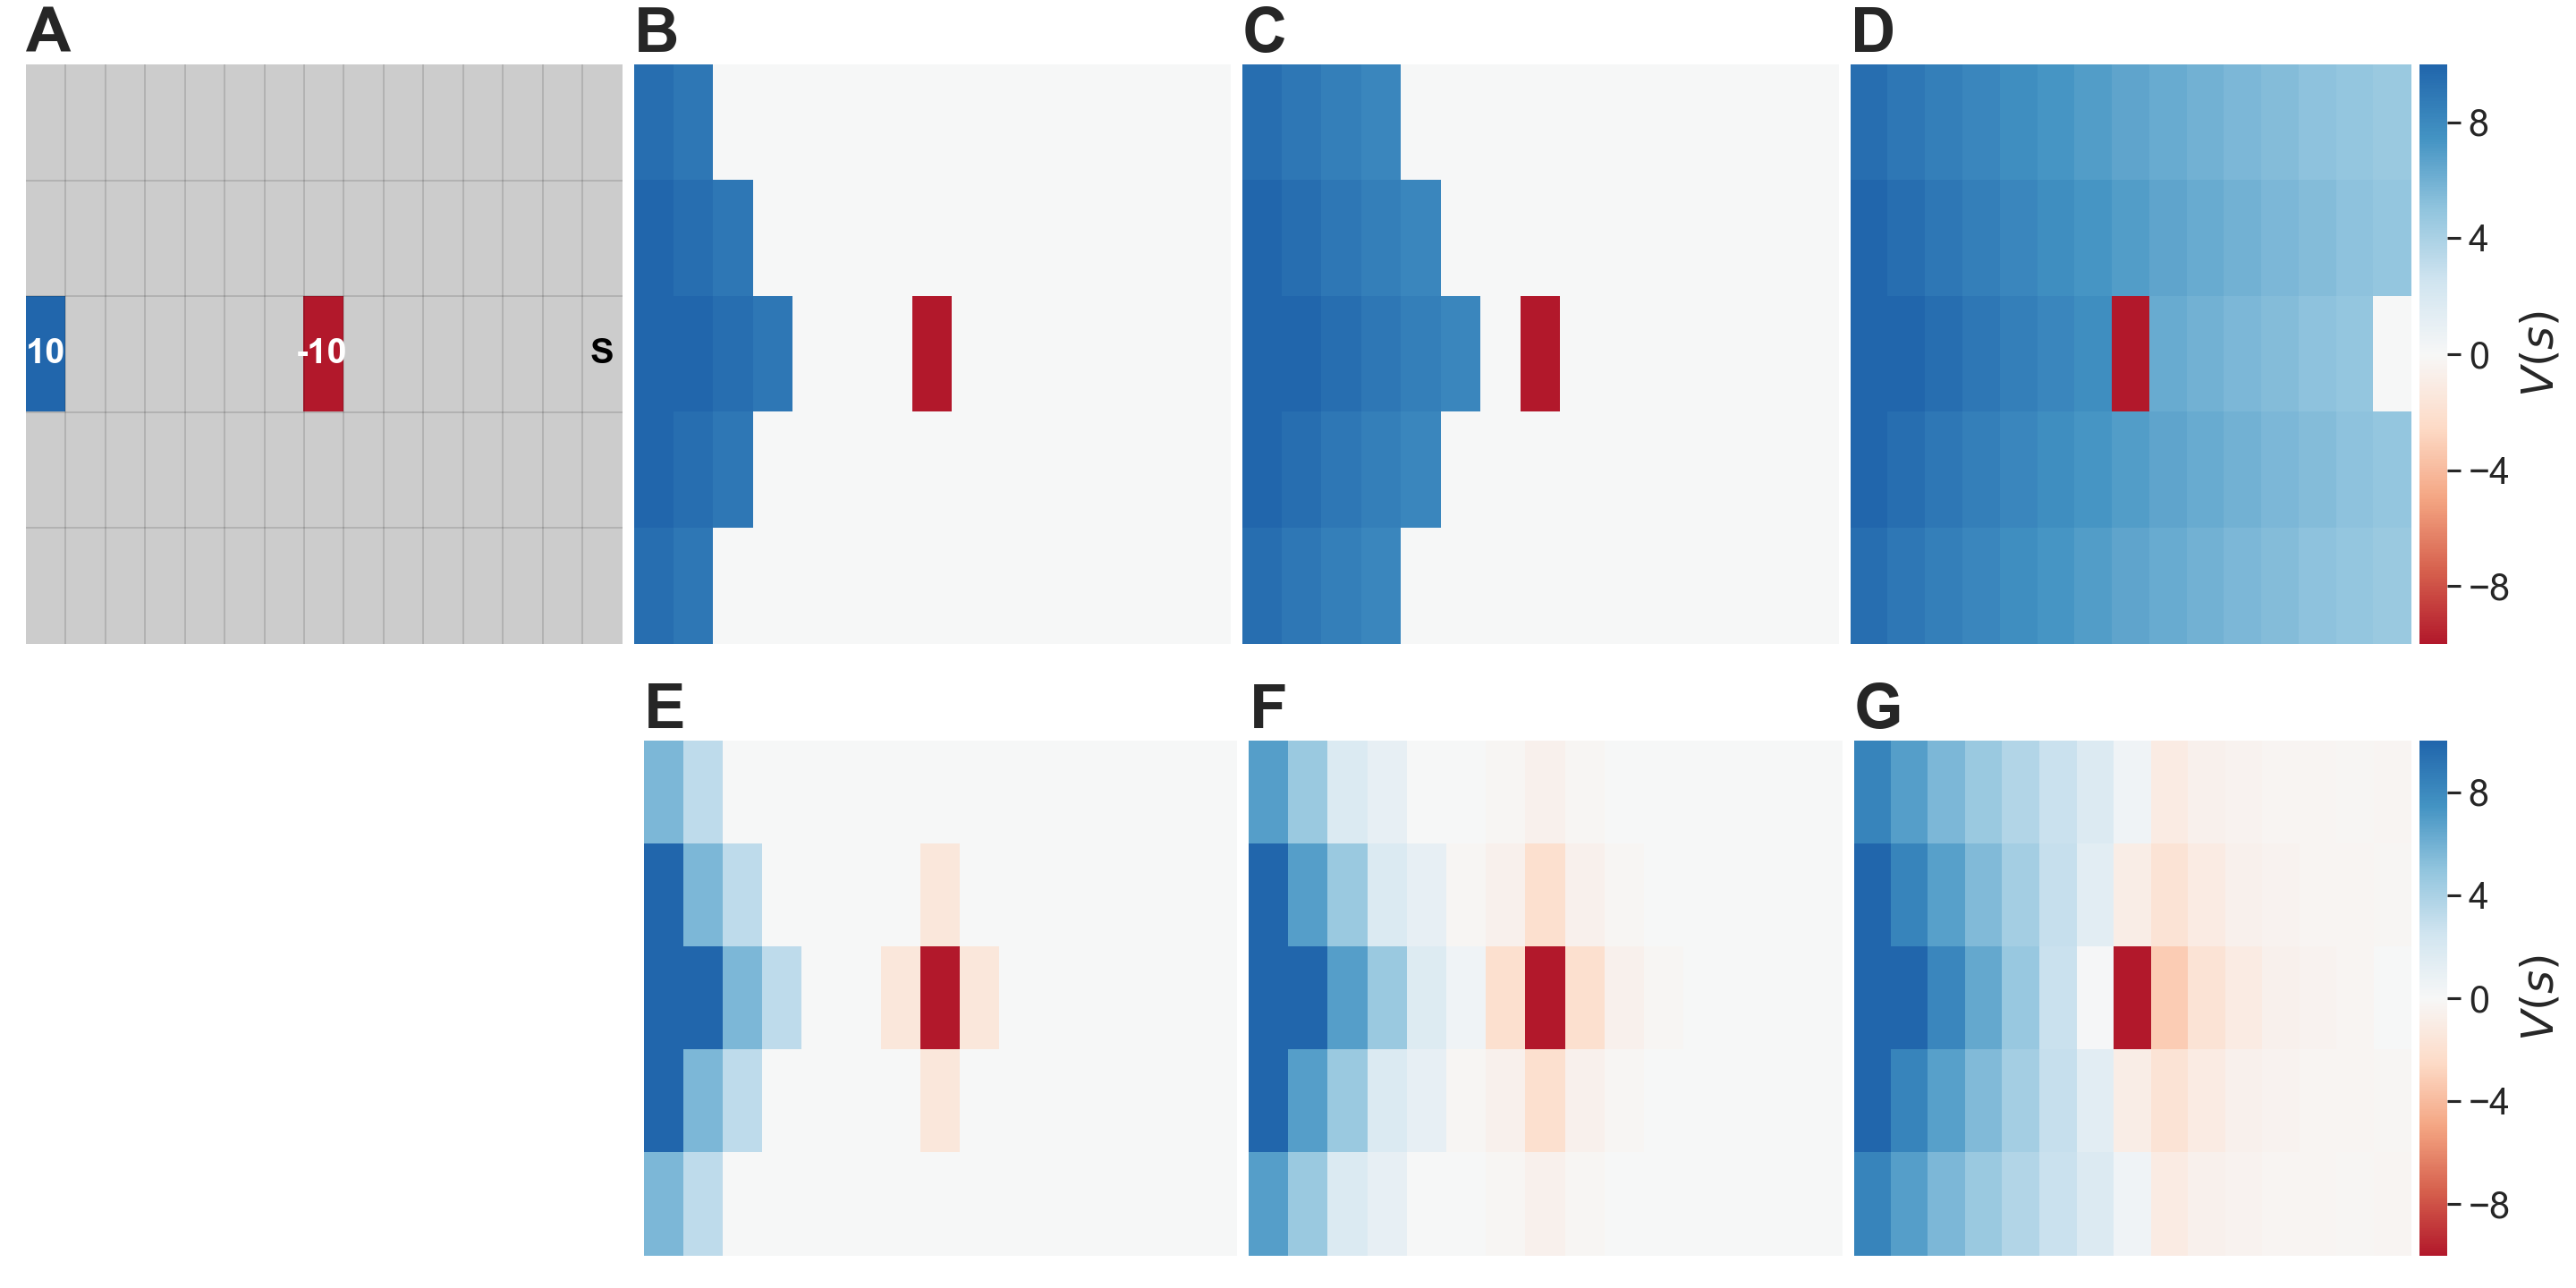
\includegraphics[trim={0 0 0 0},clip]{../figures/06_lh.png}}%
  }
  \caption{\textbf{Free Choice Premium}}
  \par remember to add parameters
\end{figure}

\section{Discussion}

All of the anxiety disorders share core symptoms including pessimistic inference,
second-order conditioning, and sustained avoidance. In this article, we offered
a simple computational account of how these aberrations may arise and be maintained.
Following the literature in Markov decision processes, we showed how a simple
breakdown in expectations about the likelihood of encountering future negative
outcomes (as a result of an unpredictable environment or unreliable policy) can
effectively backpropagate negative expectations through an agent's internal value
map. The result of which yields expectations and behaviors resembling that observed
in pathological anxiety. Importantly, we also showed that such a model can account
for aberrant behavior previously observed in individuals with anxiety in several
assays of psychiatric behavior. By no means a complete theory of anxiety, this
account helps to at least tie together several core symptoms of anxiety in one
account.

This computational account draws upon a longstanding recognition of the importance
of perceived control to the development and maintenance of anxiety disorders. Several
prominent theories of anxiety in the clinical anxiety focus on the importance of
a lack of perceived control, including helplessness-hopelessness theories, perceived
efficacy, and the triple vulnerability model. It is worth noting that that these
theories differ, among other things, in where a lack of control arises. For learned
helplessness, an agent believes to occupy an uncontrollable world; in other words,
there is no reliable mapping between action and outcome. For self-efficacy theory,
an agent believes to be limited or incapable of exerting beneficial influence on
the environment, though this is otherwise possible. Note that both can easily be
modeled in the current approach, either in the state transition function or in
future policy function. Insofar that they are multiplicative, they should result
in the same effect. Future work may tease these apart, as they may be interesting
for guiding treatment.

It is worth noting that we are not the first to attempt to formalize a theory
of control in MDP. \cite{HuysDayan2009} provided a first computational account
of learned helplessness through simple models of action-outcome contingencies.
\cite{HuysDayan2009} found that training an agent first in an unreliable environment
led to later impaired learning, akin to early learned helplessness experiments,
by virtue of the prior of controllability. This provides a nice demonstration
of learning impairment of action-outcome contingencies. Importantly, our accounts
in at least three respects. We handle sequential decision environments, which is
important as it is in sequential decision environments where the consequences
of pessimistic inference become most pronounced. Second, our account claims
that the worst outcomes are believed, wherein their account focuses on randomness.
This seems closer to the symptoms described in anxiety. Finally, our account
provides insights into maintenance. With an otherwise unmodified Bayesian learner,
their agents should eventually learn and be ok.

We discussed two mechanisms by which negative values can spread. There is a third
that we did not address here: that of the state itself. Here we assumed that states
were fully observable; in other words, there was no uncertainty about the state
an agent was currently occupying. In partially-observable Markov decision problems,
the state itself must be inferred from external and internal variables. This is
yet another means by which bad value can spread if undue likelihood is granted
to undesirable or aversive states. This ideas has previously been proposed to
explain some symptoms in anxiety \citep{Paulus2012}, and not without good reason.
Anxiety disorders involve negatively biased interpretation of ambiguous percepts
\citep{Hartley2012}, which may result in aberrant planning and increased avoidance
for similar reasons to those described above. This is an area for future research.

In this article, we have explored a computational principle of approach and
avoidance learning in sequential decision environments. We have not discussed,
however, the particular psychological or neurobiological mechanisms by which this
sort of learning may take place. This issue has been discussed in detail elsewhere
\citep{Bishop2018}, but we briefly discuss a few possibilities here. Mechanically,
we understand that complex decision problems are solved by mental processes that
exist on a spectrum between model-based and model-free (Daw et al., 2005). The
difference between these two families of methods hinges on the reliance of an
internal model of the world used to make predictions about expected long-run
outcomes of particular choices.

For model-based decision making, one possibility is biased planning. In large
state spaces, online sequential decision making suffers from the curve of
dimensionality: in planning a series of actions to take, comparing between
multiple options rapidly becomes computationally intractable when the number of
options and depth of search becomes even moderately large. Thus, heuristics for
reducing the size of this search can be useful. Biased pruning of search paths
(such as immediately discarding paths that require some minor loss in pursuit of
larger gains) may result in maladaptive decision making (Huys et al., 2012).
Alternately, if planning relies on internal sampling from previously experienced
episodes in order to make predictions about future value, then biased sampling
may similarly result in maladaptive decision making. Recent work has shown how
finite sampling during planning can result in risk aversion and the overrepresentation
of low probability but strongly negative outcomes (Lieder et al., 2018). Such a
mechanism is prima facie in line with results showing the availability in memory
of negative outcomes being higher for patients with anxiety (Borkovec et al., 1999;
Miranda and Mennin, 2007).

Within the realm of model-free decision making, several studies have found evidence
suggesting increased learning rates for negative reward prediction errors in
individuals with elevated levels of anxiety \citep{Aylward, Huang2017, Harle2017
garrett2018}. Though an asymmetry in sensitivity to
positive and negative reward prediction errors bears superficial similarity, for
the reasons described above merely attending more to negative information does not
necessarily predict increased avoidance insofar that avoidance can successfully
isolate negative outcomes. One possibility, and topic of future research, is how
prior beliefs about the reward statistics of the current environment dictate
learning rates. A second possibility is prioritized replay (Russek et al., 2017;
Mattar and Daw, 2018). Offline replay of previous experiences (through hippocampal
mechanisms) are known to facilitate learning. It has been proposed that biased
replay could bias value estimates (Gagne et al., 2018). This is another exciting
area for future research.


\bibliographystyle{vancouver-authoryear}
\bibliography{citations}

\section{Appendix}

\begin{algorithm}
  \caption{Value Iteration}

  \State Algorithm parameter: a small threshold $\theta > 0$ determining accuracy of estimation
  \State Initialize $V(s)$, for all $s \in S$ arbitrarily, except that $V(terminal) = 0$
  \State
  \While{$\Delta > \theta$}
    \State $\Delta \leftarrow 0$
    \Loop \ for each $s \in S$
      \State $v \leftarrow V(s)$
      \State $ V(s) = \max_a \sum_{s',r} p(s',r|s,a) \left[ r + \gamma V(s') \right] $
      \State $\Delta \leftarrow \max(\Delta, |v - V(s)|)$
    \EndLoop
  \EndWhile

\end{algorithm}

\end{document}
